\documentclass[a0paper]{tikzposter}

\usetheme{Steph}

% Packages
\usepackage[T1]{fontenc}
\usepackage[utf8]{inputenc}
\usepackage{natbib,mdframed,amsmath,calc,graphicx,amssymb,relsize,multirow,rotating,bm,url,multicol,array,subfigure,eurosym}
\usepackage{tikz}
\usetikzlibrary{arrows,patterns, calc, arrows.meta}
\tikzset{>={Latex[width=3mm,length=5mm]}}

\renewcommand{\rmdefault}{phv}
\renewcommand{\sfdefault}{phv} 
\renewcommand{\labelitemi}{$\bullet$}

\newcommand{\compresslist}{
    \setlength{\itemsep}{1pt}
	\setlength{\parskip}{0pt}
	\setlength{\parsep}{0pt}
}

\definecolor{IGNVert}{RGB}{163, 210,  11}
\definecolor{IGNGris}{RGB}{159, 164, 168}
\definecolor{IGNGrisFonce}{RGB}{101, 105, 110}



\title{Simulation models for systems of cities and sustainable development goals}
\author{Juste Raimbault$^{1, 2, \ast}$, Denise Pumain$^{2}$}
\institute{$^{1}$ LASTIG, Univ. Gustave Eiffel, IGN-ENSG\\
$^{4}$ UMR CNRS 8504 G{\'e}ographie-cit{\'e}s\\\vspace*{0.5em}
$^{\ast}$ \texttt{juste.raimbault@ign.fr}
}
\titlegraphic{}

\makeatletter
\renewcommand\TP@maketitle{
    \hspace{-.12\textwidth}
	\begin{tabular}{lcl}
	%logo box 1
        
    	\begin{minipage}[b][.1\textheight][b]{.15\textwidth}
      
        	
\includegraphics[width=0.7\linewidth]{./figures/LOGO_IGN}\\
            
             \vspace{1cm}
            
            
\includegraphics[width=0.7\linewidth]{./figures/lastig}
    	\end{minipage}
    	&
    	%title box
    	\begin{minipage}[b][.1\textheight][b]{.6\textwidth}

            
     
    		\centering
    		\color{titlefgcolor}
            \vspace{1cm}
    		%{\bfseries \Huge \sc \@title \par}
    		
    		{\bfseries \Huge \sc Simulation models for systems of cities and \par}

      {\bfseries \Huge \sc sustainable development goals \par}
      
    		\vspace*{2em}
    		{\huge \@author \par}
    		\vspace*{1em}
    		{\LARGE \@institute}
    		
    	\end{minipage}
    	&
    	%logo box 2
    	\begin{minipage}[b][.1\textheight][b]{.15\textwidth}
            	
\includegraphics[width=1\textwidth]{./figures/ccs2024_logo_transparent}
             
             \vfill
             \vfill
     
     \end{minipage}
     
	\end{tabular}
}
\makeatother

%%%%%%%%%%%%%%%%%%%%%%%%%%%%%%%%%%%%%%%%%%%%%%%%%%%%%%%%%%%%%%%%%%%%%%%%%%%%%%%%
% Multicol Settings
%%%%%%%%%%%%%%%%%%%%%%%%%%%%%%%%%%%%%%%%%%%%%%%%%%%%%%%%%%%%%%%%%%%%%%%%%%%%%%%%
\setlength{\columnsep}{1.5em}
\setlength{\columnseprule}{0mm}

%%%%%%%%%%%%%%%%%%%%%%%%%%%%%%%%%%%%%%%%%%%%%%%%%%%%%%%%%%%%%%%%%%%%%%%%%%%%%%%%
% Save space in lists. Use this after the opening of the list
%%%%%%%%%%%%%%%%%%%%%%%%%%%%%%%%%%%%%%%%%%%%%%%%%%%%%%%%%%%%%%%%%%%%%%%%%%%%%%%%


% To remove the "latex tikz poster" at the bottom right corner
\tikzposterlatexaffectionproofoff

\begin{document}
	% Title block with title, author, logo, etc.
	\maketitle
	
%------------------------------------------------------
%----------------LINE 1--------------------------------
%------------------------------------------------------
% block alone on its line so you don't have to specify the columns environment

\vspace*{-5cm}

		%==============================================
		\block[titlewidthscale=0.5]{Sustainability trade-offs in systems of cities}{

            %Cities are at the core of sustainability issues, as they can have an equally positive or negative impact on several dimensions of sustainable development goals: for example urban sprawl will increase land uptake and transport emissions while on the contrary urban densification will increase accessibility and mitigate land-use change \cite{naess2020urban}; urban segregation emerges in many contexts, but cities remain vectors of equity and equal access to opportunities \cite{vaughan2011challenges}; cities are incubators of innovation and social change \cite{pumain2008socio}, but this may increase subsequent economic activities and emissions. These apparent contradictions are a product of the high complexity of urban systems, and understanding trade-offs and synergies between sustainable development goals (SDGs) in urban system requires a complex systems approach \cite{zhao2021synergies}.

            $\rightarrow$ urban systems induce both negative and positive externalities on many sustainability dimensions, leading to trade-offs between sustainable development goals \cite{zhao2021synergies}

            \bigskip

            $\rightarrow$ simulation models for systems of cities at a macro scale are a tool to quantify and understand these \cite{raimbault2022trade}

            % This contribution develops recent developments to simulation models for systems of cities applied to the quantification of SDGs related to urban dynamics at the macroscopic scale. 

            \bigskip
            \bigskip

            \textbf{Research objective:} develop a multi-model integrating several SDG dimensions to study and optimise many-dimensions trade-offs
   
		}
		%==============================================

  

	
	%==============================================
	\block[titlewidthscale=0.5]{Multi-modelling urban dynamics at the macro scale}{

            % Building on the series of Simpop models \cite{pumain2011multi}, a model of urban evolution was applied by \cite{raimbault2022trade} to find trade-offs between innovation within cities and their emissions. This model was extended to include further dimensions of SDGs by \cite{raimbault2022complex}, including economic performance, economic inequalities, and the development of infrastructure. The corresponding coupled submodels are a model of innovation diffusion, a model of economic exchanges, and a model of transport network and cities co-evolution.

 
		\begin{minipage}{0.5\textwidth}

                $\rightarrow$ based on Simpop models \cite{pumain2011multi}, cities populations are simulated on long time scales (100years) and small spatial scales (systems of cities) based on \textbf{spatial interactions} and \textbf{other dimensions captured by submodels} \cite{raimbault2021spatial}:

                \medskip

                \begin{itemize}
                    \item the hierarchical diffusion of innovations \cite{raimbault2020model}
                    \item economic exchanges between cities \cite{cottineau2015modular}
                    \item the co-evolution between cities and the interurban transport network \cite{raimbault2021modeling}
                \end{itemize}

                \bigskip
                \bigskip

                $\rightarrow$ indicators quantifying sustainability regarding different goals: utility of innovations (SDG 9), transport emissions (SDG 13), transport infrastructure (SDG 9), economic inequalities (SDG 10), wealth (SDG 8)


                % Setup and implementation
   
            \end{minipage}\hfill
		\begin{minipage}{0.2\textwidth}

            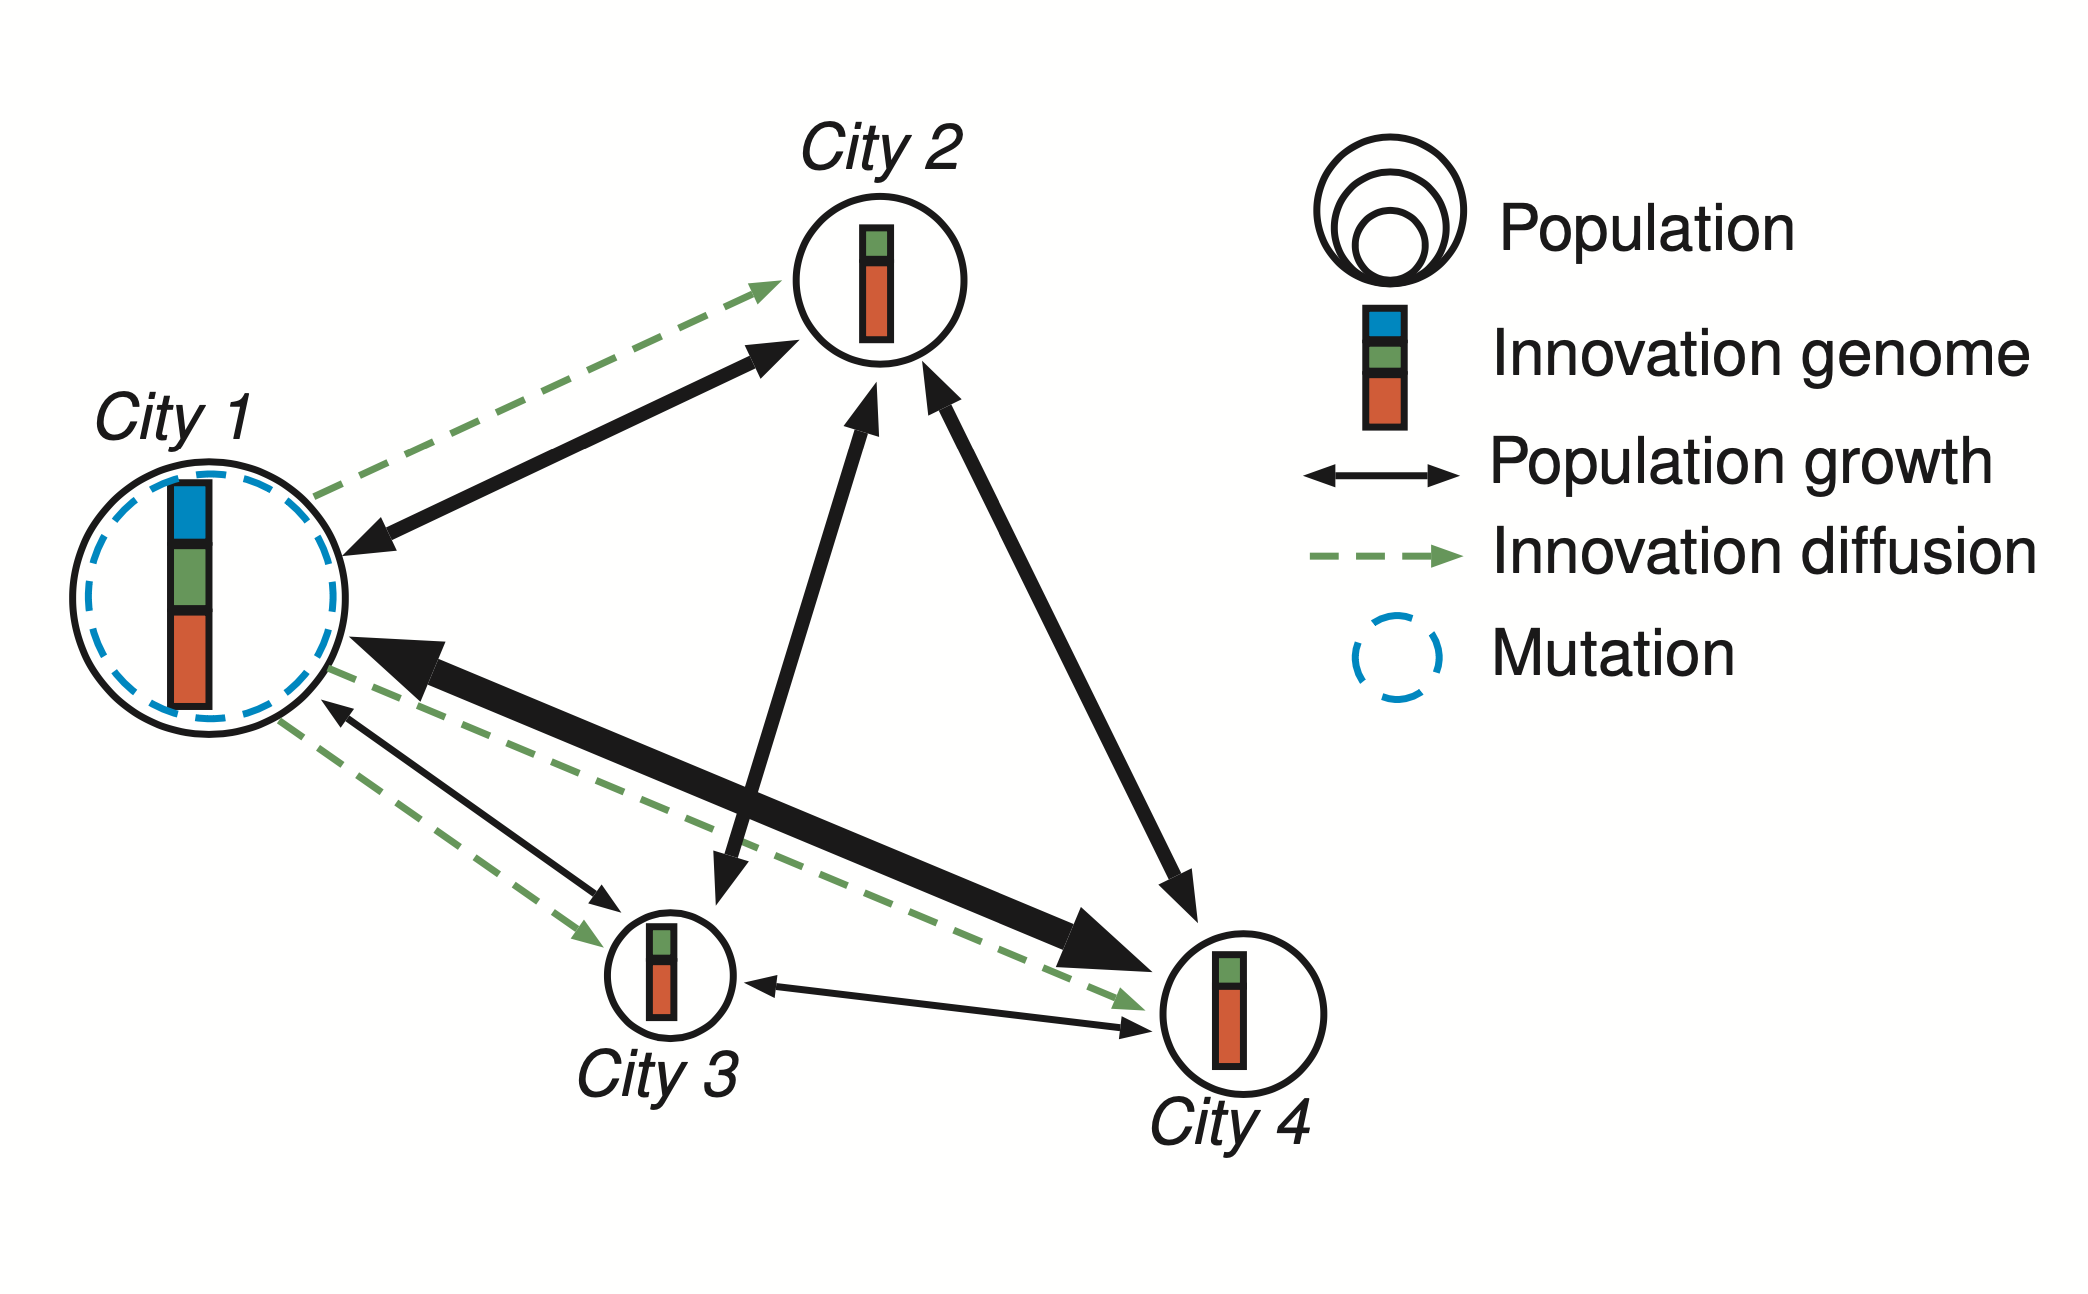
\includegraphics[width=\linewidth]{figures/model_4.png}

            \medskip

            \textit{Processes of spatial interaction and innovation diffusion for the innovation submodel}
   
		\end{minipage}\hfill%\vrule
            \begin{minipage}{0.12\textwidth}

%            \begin{multline}
%S_0 \rightarrow \left[ S_1^{(0)} = M_0 (S_0) \rightarrow \ldots \\
%\rightarrow S_1^{(K - 1)} = M_{K - 1} (S_1^{(K - 2)}) = S_1 \right] \longrightarrow \ldots \\
%\longrightarrow \left[ S_{T}^{(0)} = M_0 (S_{T - 1}) \rightarrow \ldots \\
%\rightarrow S_T^{(K - 1)} = M_{K - 1} (S_T^{(K - 2)}) = S_T \right]
%\end{multline}

\[
\begin{cases}
    S_0^{(t)} = S_t \\
    S_{k+1}^{(t)} = M_{k}\left[S_{k}^{(t)} \right] \\
    S_{t+1} = S_{K}^{(t)}
\end{cases}
\]

            \bigskip
            \bigskip

            \textit{Sequential coupling of $K$ submodels at each time step $t$}

            \end{minipage}
		
	}


        

         

		%==============================================
		\block[titlewidthscale=0.5]{Application: SDG trade-offs in 5 dimensions}{

            \begin{minipage}{0.55\textwidth}
                
                $\rightarrow$ application to many-dimensions optimisation of indicators in synthetic systems of cities

                \bigskip

                $\rightarrow$ model implemented in scala within the \texttt{spatialdata} library \cite{raimbault2020scala}

                 \bigskip

                 $\rightarrow$ integration into the OpenMOLE software for model exploration and validation \cite{reuillon2013openmole}

                 \bigskip

                 $\rightarrow$ many-objective optimisation in 5 dimensions, using the NSGA2 genetic algorithm to obtain Pareto fronts, which provide trade-offs between the SDG indicators

                 \bigskip

                \begin{center}
                    
\includegraphics[width=0.1\linewidth]{figures/iconOM.png}
                    
\includegraphics[width=0.3\linewidth]{figures/openmole.png}
                \end{center}
            
            \end{minipage}\hfill
            \begin{minipage}{0.2\textwidth}
                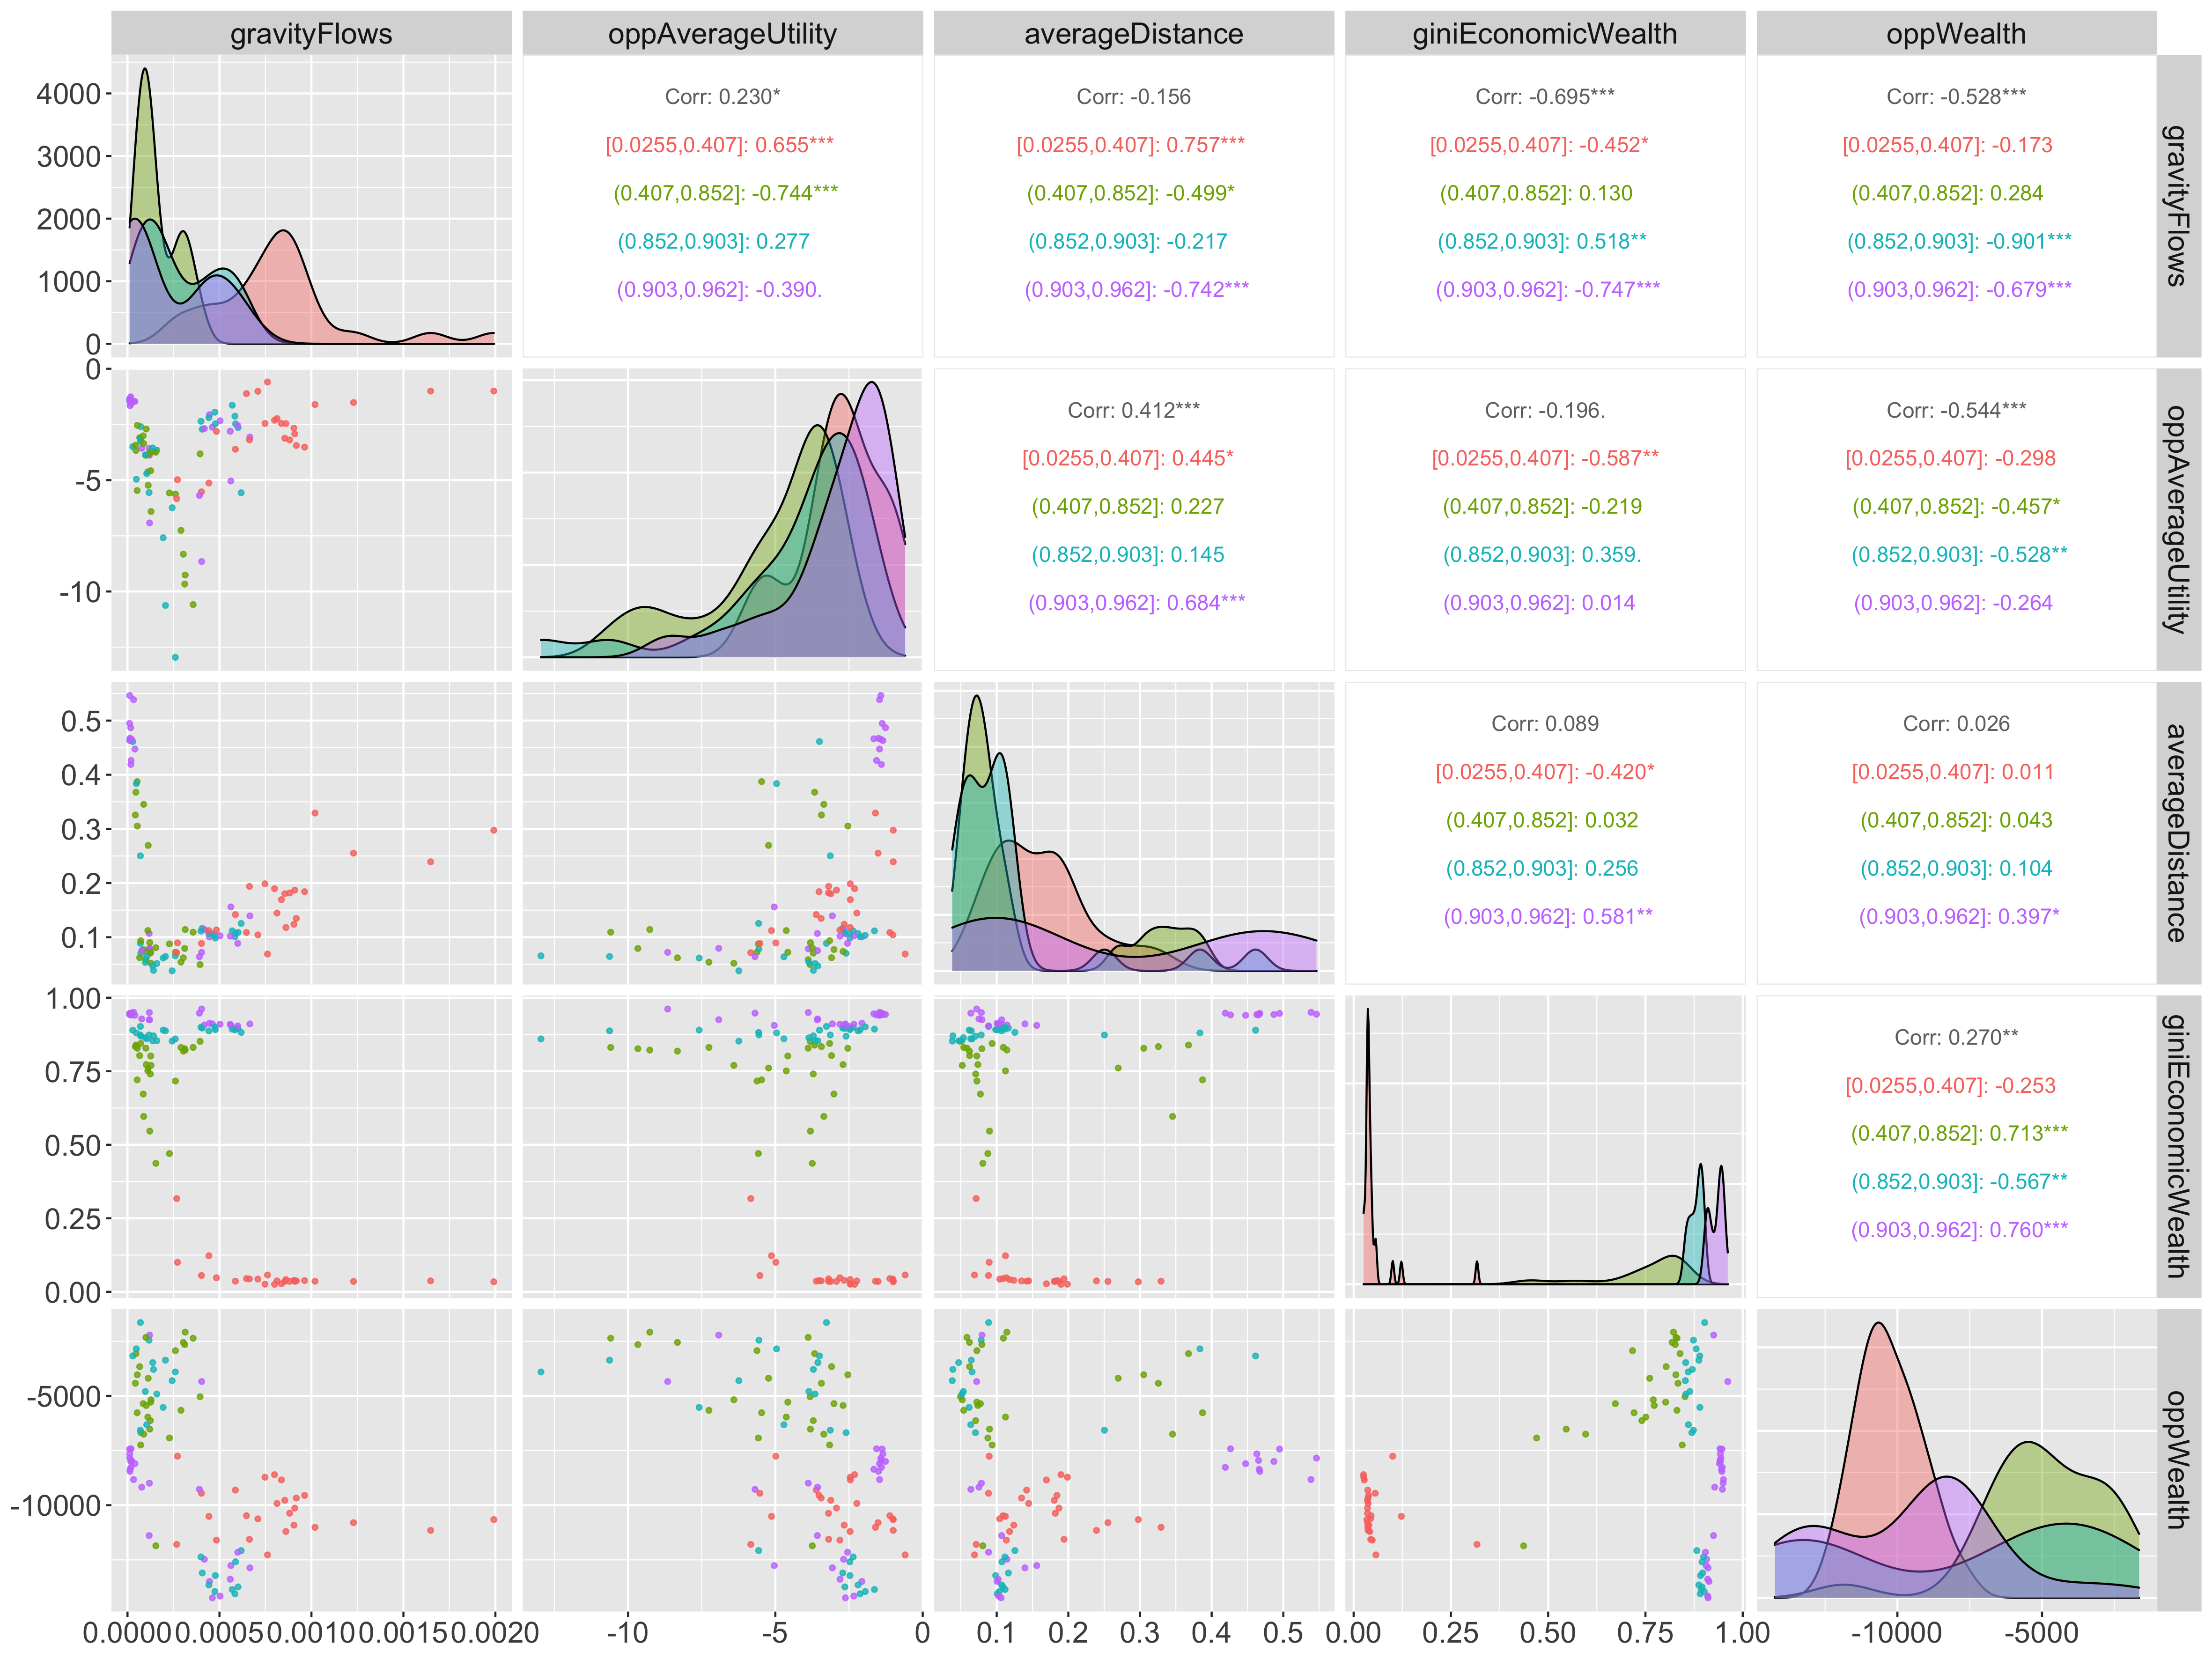
\includegraphics[width=\linewidth]{figures/scatter_models_colorginiEconomicWealth_OPTIMISATION_GRID_20220622_092133.png}
            \end{minipage}\hfill
            \begin{minipage}{0.15\textwidth}
                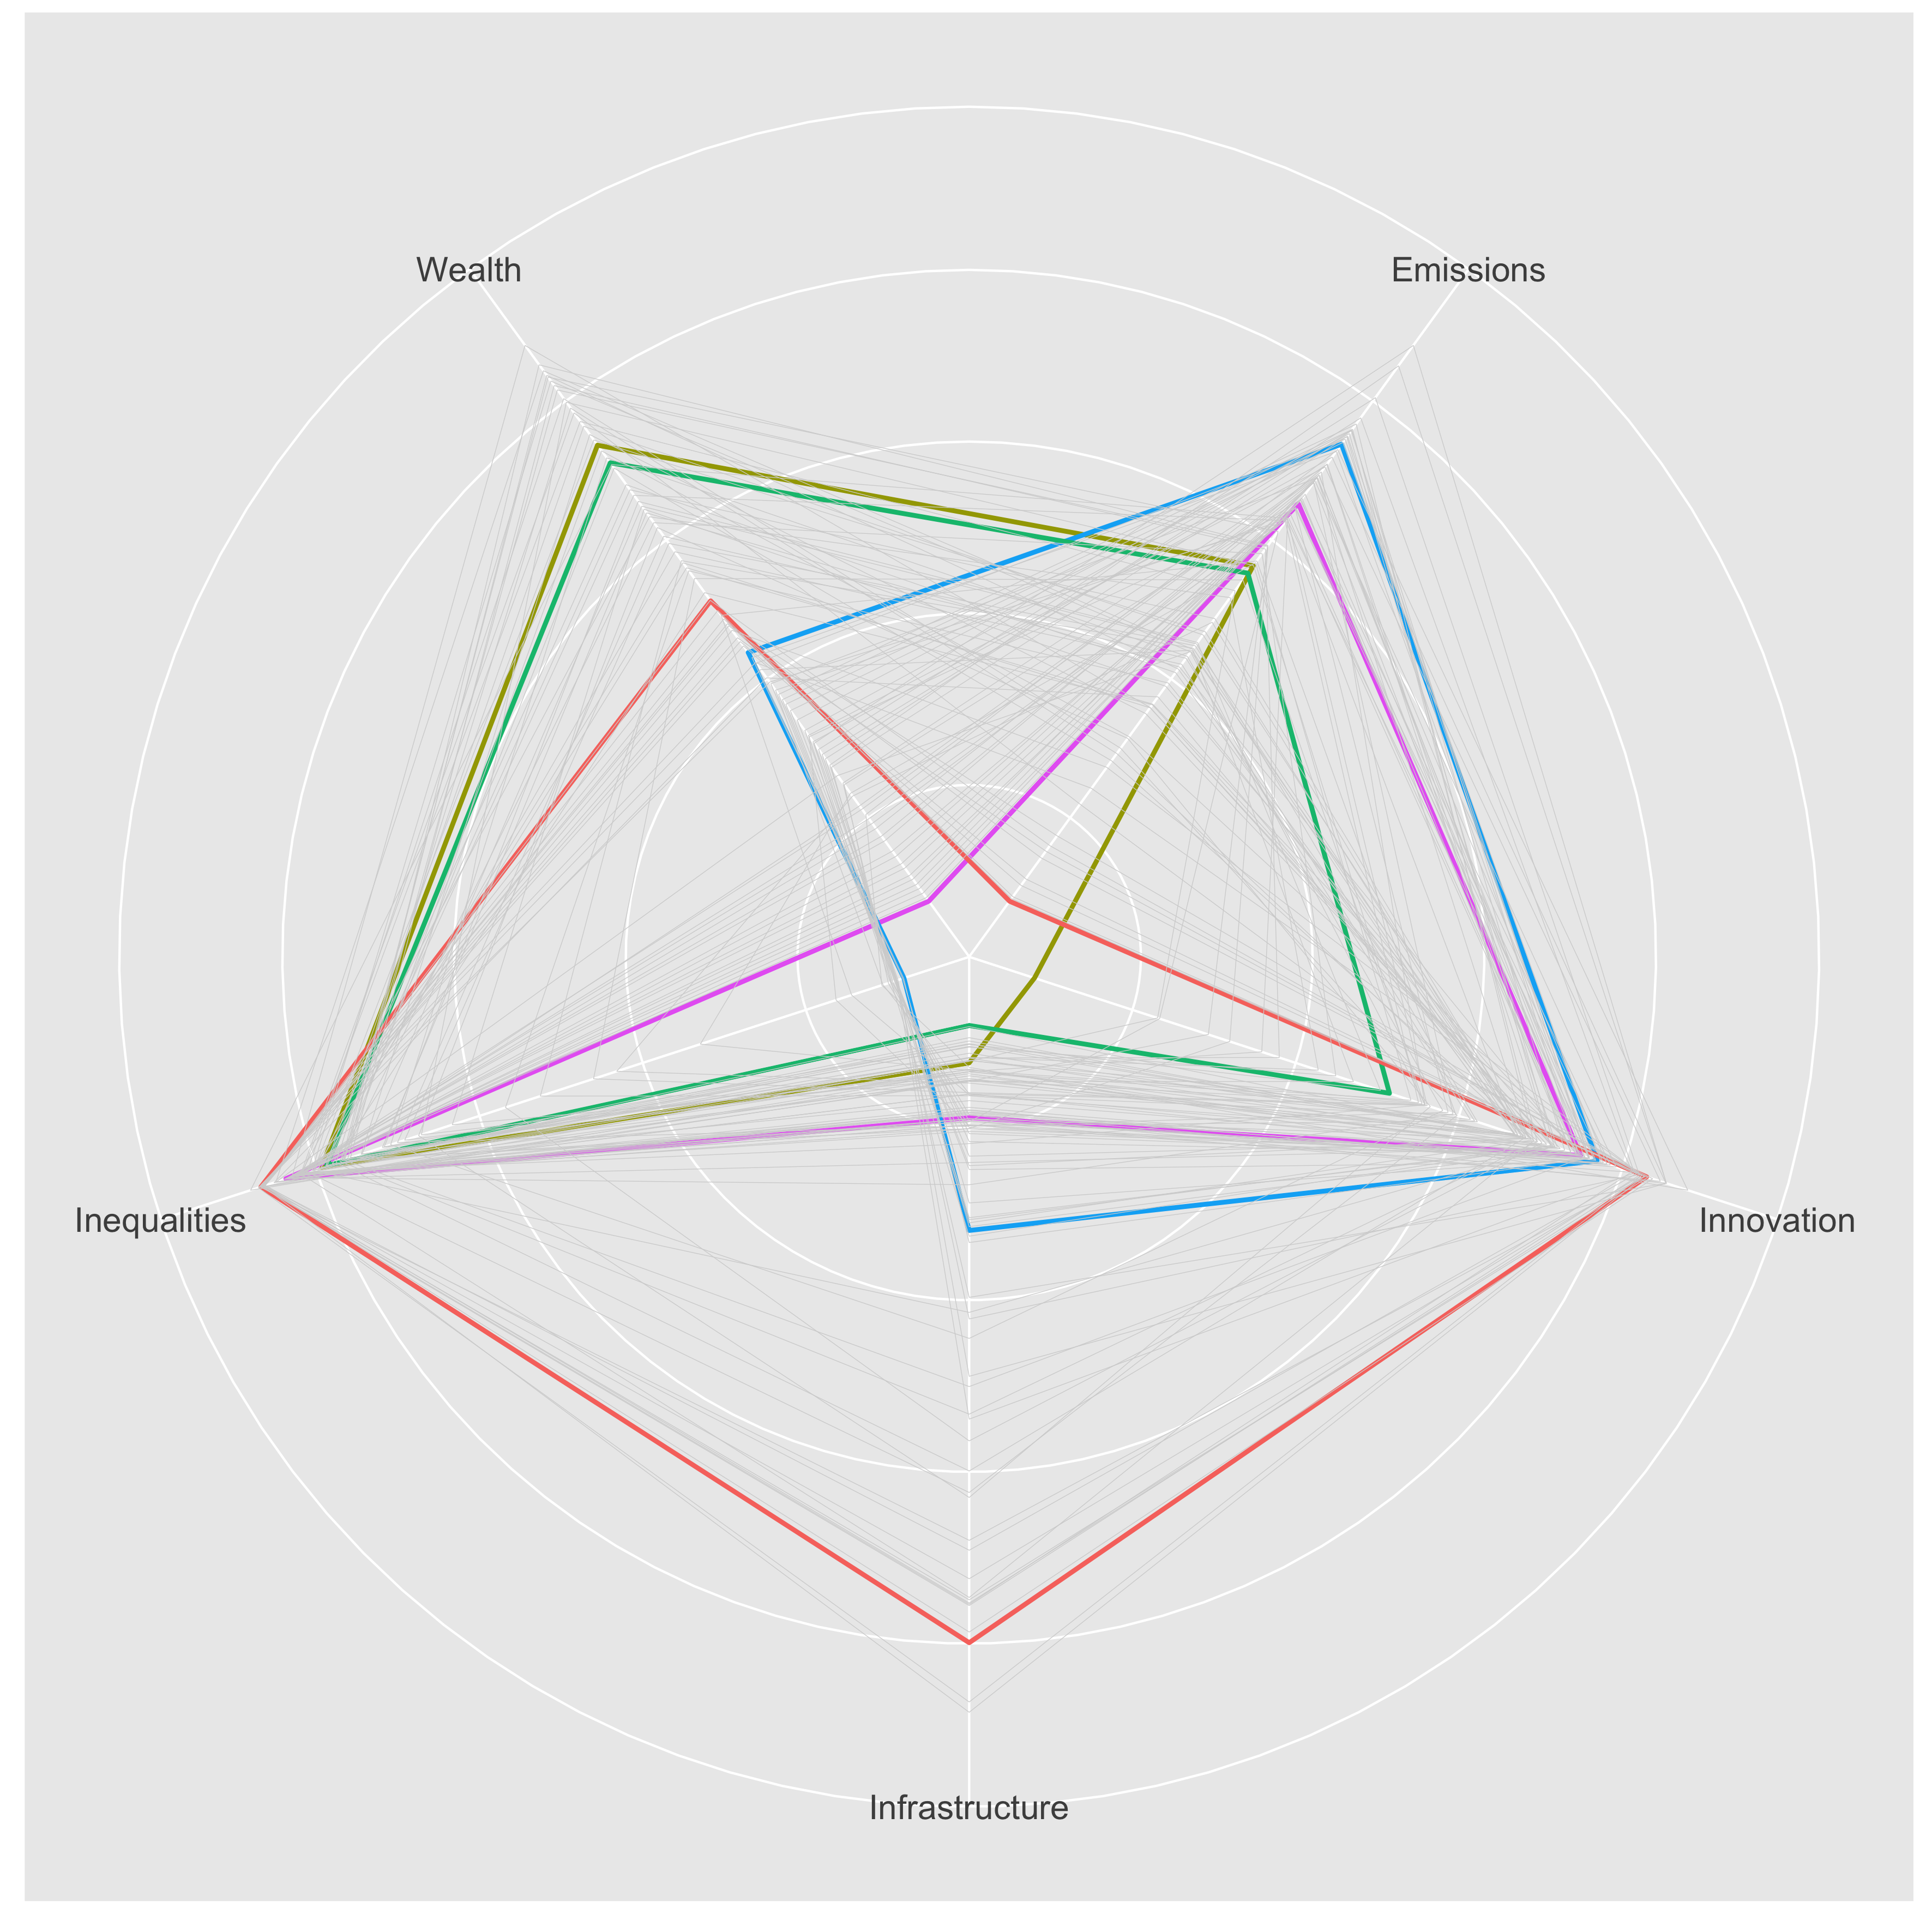
\includegraphics[width=\linewidth]{figures/radar_sdgs.png}
            \end{minipage}

   
		}

        \block[titlewidthscale=0.5]{Developments in progress for model validation}{


%Our first development is to better understand how coupling choices between submodels has a role to play in emergent dynamics. The previous version of the model only included a sequential coupling between submodels at each time step, and no strong coupling in the sense of reciprocal feedback loops. We test a version with such strong coupling, where two components (for example innovation and infrastructure) are strongly coupled, and the remaining components are used upstream only to compute the corresponding SDGs. All possible couples among submodels were tested, and we find significantly different trajectories between these combinations and with the sequential implementation.

\textbf{Question 1: \textit{how does the type of coupling for submodels influence emergent dynamics?}} 

\bigskip

$\rightarrow$ comparison between strong couplings of submodels (all combinations of submodels in a sequential coupling) with weak couplings (one main model and other submodels only downstream to compute indicators without influencing population dynamics) 

\bigskip
\bigskip
\bigskip



%Our second development is the quantification of strong emergence in the simulated dynamics. Following \cite{raimbault2023innovation} which applied the method developed by \cite{rosas2020reconciling} on a multi-scale model of innovation dynamics within systems of cities, we use the same indicators to measure if our urban dynamics model effectively captures strong emergence. Some parameter regimes indeed simulate strongly emergent dynamics, meaning that in some cases the macro state of the urban systems has some causal influence on the trajectories of single cities.

\textbf{Question 2: \textit{do the simulated dynamics capture strong emergence?}} 

\bigskip

$\rightarrow$ \cite{raimbault2023innovation} applied information theory indicators proposed by \cite{rosas2020reconciling} on a multi-scale model of innovation dynamics and found a large set of emergence regimes with a diversity search algorithm; application of the same approach to the macro-scale multi-model

\bigskip
\bigskip
\bigskip

%Our third development is the parametrisation of the model on a real world configuration, as previous results were obtained for synthetic systems of cities. We consider the Chinese system of cities between 1980 and 2010. Using the database of \cite{swerts2017data} for population, we initialise the model with populations, and try to calibrate the model by fitting simultaneously population time-series for all cities, and the 2010 state for other dimensions (emissions, innovation measured by patents, GDP). We find that it remains difficult to have a good performance on all dimensions, suggesting that further work in the coupling specification should be done, possibly the construction of a more complex model with a stronger integration between the different components.

\textbf{Question 3: \textit{how to apply the model to a real system of cities?}} 

\bigskip

$\rightarrow$ setup on the Chinese system of cities between 1980 and 2010 using data by \cite{swerts2017data} for populations, and GHSL for emissions and GDP; calibration on population trajectories


\bigskip
\bigskip
\bigskip

%These preliminary results confirm that constructing a model that simulates different dimensions of SDGs in systems of cities is difficult, since many diverging model versions are possible and that calibration does not identify a single best model version. These models however capture strong emergence in some case and thus some complexity of these urban systems. Future work will have to understand more systematically how model coupling plays a role in that context, and to built better real-world parametrisation on different systems of cities.

\textbf{Future work: } towards models applied to multi-scalar policy-making, requiring an extensive validation and understanding of model behaviour, and robust parametrisations on real-world systems
   
		}
		
	%==============================================
		% bibliography managed with natbib
		\block[titlewidthscale=0.2,bodyoffsety=1.8cm,titleoffsety=.1cm]{References}{
			% This command is to prevent the printing of a second "références" in text and to delete white space between block title and bibliography
			\renewcommand\refname{\vskip -2cm}
			% Bibliography input. 
			%Refrences should be added directly to the Biblio.bib file. Refrences should in bibTex Format. Every Reference cited in the poster will be automatically added.
            %\footnotesize
            \small
   
			\bibliography{biblio}
			% Plain style so that cited articles appear as number in the poster and are only fully displayed here
			\bibliographystyle{plain}
		}
	    %==============================================	

		
	
	
\node [above right,outer sep=20pt,minimum width=\textwidth,align=center,draw=none,fill=none, text = IGNGrisFonce] at (bottomleft) {\centering \huge \bf Conference on Complex Systems 2024, Exeter, September 2nd-6th 2024};


\end{document}

\endinput




	

\begin{columns}
		
	

% Template


			\vspace{.5cm}
			
			%This block contain example of Tikz
			
			\centering
			
			\begin{tikzpicture}[scale=2]
			\draw[-latex] (0,0) -- (0,3.2);
			\draw[-latex] (0,0) -- (5.2,0);
			\node at (-0.2,1.5) {$\theta$};
			\node at (2.5,-0.2) {$\mathit{t}$};
			
			\node at (0.2,0) {$\bullet$};
			\node at (0.4,0.8) {$\bullet$};
			\node at (0.6,1.6) {$\bullet$};
			\node at (0.8,2.4) {$\bullet$};
			\node at (1.8,0.4) {$\bullet$};
			\node at (2,1.2) {\textcolor{red!60!black}{$\bullet$}};
			\node at (2.2,2) {$\bullet$};
			\node at (2.4,2.8) {$\bullet$};
			\node at (3.4,0) {$\bullet$};
			\node at (3.6,0.8) {$\bullet$};
			\node at (3.8,1.6) {$\bullet$};
			\node at (4,2.4) {$\bullet$};
			
			\draw[->,red!60!black] (2,1.2) -- (0.4,0.8);
			\draw[->,red!60!black] (2,1.2) -- (0.6,1.6);
			\draw[->,red!60!black] (2,1.2) -- (1.8,0.4);
			\draw[->,red!60!black] (2,1.2) -- (2.2,2);
			\draw[->,red!60!black] (2,1.2) -- (3.6,0.8);
			\draw[->,red!60!black] (2,1.2) -- (3.8,1.6);
			\end{tikzpicture}
			
			Exemple de Tikz 

			\vspace{.5cm}
			


